\section{RISMC approach to multi-unit modeling}
\label{sec:RISMC_MU_modeling}

This section shows in detail how the actual multi-unit model has been implemented
using RAVEN and RELAP5-3D. 

\begin{figure}
    \centering
    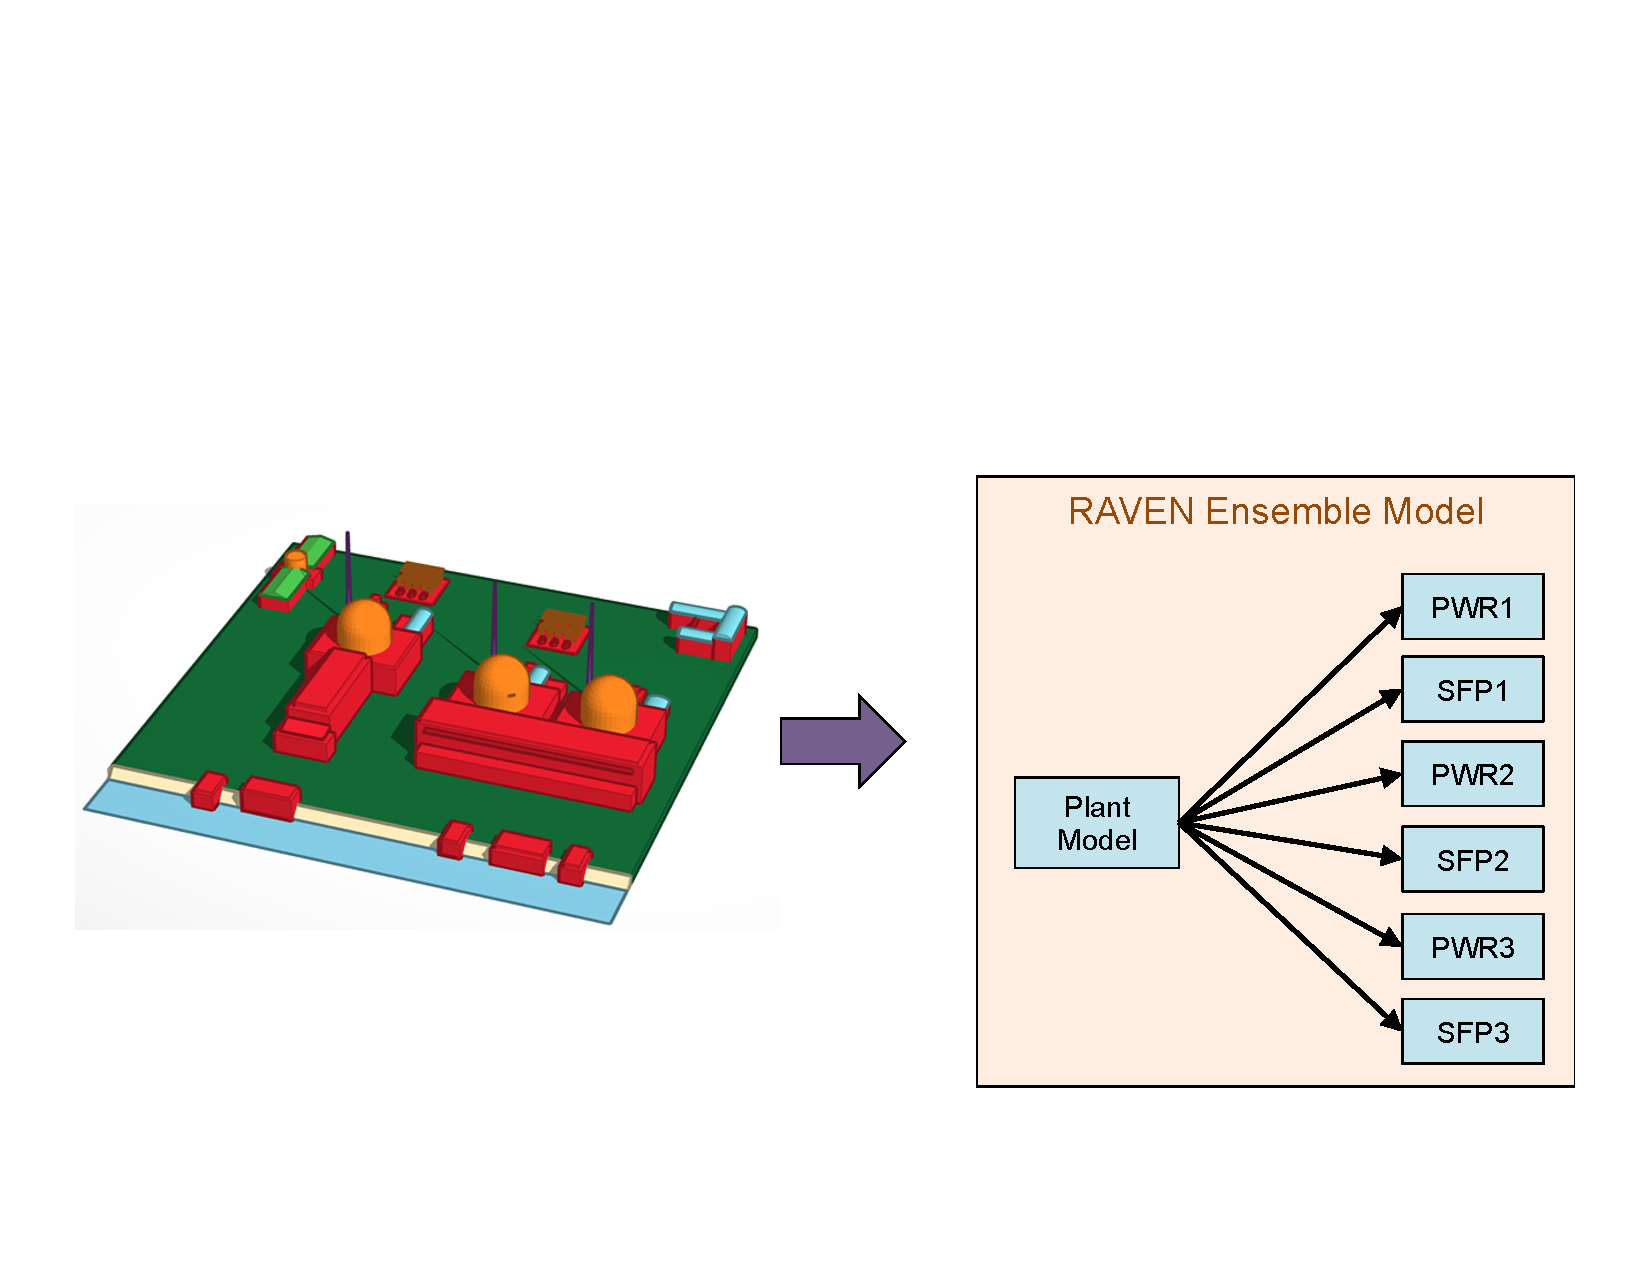
\includegraphics[scale=0.5]{ensembleModel.pdf}
    \caption{RAVEN ensemble model for the considered test case}
    \label{fig:ensembleModel}
\end{figure}

\subsection{System Models}
[CARLO]
\subsubsection{PWR1 and PWR3}

\subsubsection{PWR2}

\subsubsection{SFPs}

\subsubsection{Human models}
[RON]

\subsection{Plant Model}
The plant model has been coded as a Python script and interfaced with RAVEN as an 
external model. Its main purpose is to determine timing and sequencing of events 
for all six system models (i.e., PWRs and SFPs) given the sampled values of the 
stochastic parameters.

\subsection{Plant Stochastic Modeling}
We have identified 23 stochastic parameters 

A summary of the chosen stochastic parameters are listed in Table~\ref{tab:stochasticParameters} 
along a description and with their probabilistic distribution.

\begin{table}
  \begin{center}
      \begin{tabular}{ | l | p{5cm} | p{5cm} |}
        \hline
        Parameter          & Distribution & Description       \\ \hline \hline
        AUXFWxtieTime      &              & Time to perform AFW cross-tie  \\ \hline
        CSTxtieTime        &              & Time to perform CST cross-tie \\ \hline
        recoveryStrategy   &              & Recovery strategy to be followed   \\ \hline
        EPETime1           &              & Time to connect EPE to Unit 1   \\ \hline
        EPETime2           &              & Time to connect EPE to Unit 2   \\ \hline
        EPEime3            &              & Time to connect EPE to Unit 3   \\ \hline
        EDGSinvolAlign     &              & Probability of occurrence for EDGS involuntary alignment   \\ \hline
        EDGSinvolAlignTime &              & Time of occurrence for EDGS involuntary alignment   \\ \hline
        EDGSswitchTime     &              & Time required to change EDGS alignment   \\ \hline
        ACxTieUnit12       &              & Time to perform AC cross-tie   \\ \hline
        batteryTime1       &              & Battery life for Unit 1   \\ \hline
        batteryTime3       &              & Battery life for Unit 3   \\ \hline
        locaTimePWR1       &              & Time of occurrence for PWR1 seal LOCA   \\ \hline
        locaTimePWR3       &              & Time of occurrence for PWR3 seal LOCA   \\ \hline
        locaSizeSFP1       &              & LOCA size for SFP1   \\ \hline
        locaSizeSFP2       &              & LOCA size for SFP1   \\ \hline
        locaSizeSFP3       &              & LOCA size for SFP1   \\ \hline    
        locaTimeSFP1       &              & Time of occurrence forSFP1 LOCA   \\ \hline
        locaTimeSFP2       &              & Time of occurrence forSFP2 LOCA  \\ \hline
        locaTimeSFP3       &              & Time of occurrence forSFP3 LOCA   \\ \hline
        flex3Strategy13    &              & Rain will still   \\ \hline
        flex3Strategy2     &              & Rain will still   \\ 
        \hline
      \end{tabular}
  \end{center}
  \label{tab:stochasticParameters}
\end{table}


